\chapter{Localization}
\label{ch:localization}

\pkg{dharma_localization} bridges the LiDAR-inertial odometry into the REP-105 tree and keeps
\frm{map}$\to$\frm{odom} with an extended Kalman filter. A map's frame is the frame its fiducials
were recorded in: a tag in view puts the robot back on that map wherever it starts. Any marker
detector works as long as it puts the marker frames under the camera optical frame on TF
(\code{apriltag_ros} today~\cite{olson2011apriltag,wang2016apriltag2}).

\section{Gravity-aligned bridge}
\label{sec:leveling}

The node publishes two static transforms:
\begin{equation}
  \T{odom}{ci} = L\, \T{base}{imu}, \qquad \T{body}{base} = \big(\T{base}{imu}\big)^{-1},
\end{equation}
so that $\T{odom}{base} = L\, \T{base}{imu}\, \T{ci}{body}(t)\, \T{imu}{base}$ equals $L$ at start
(where $\T{ci}{body} = \mathbf{I}$).

\textbf{Levelling.} Standing still, the accelerometer measures the reaction to gravity, a vector
pointing up in the IMU axes. Over a still window (1~s, angular rate below 3°/s, spread of the
specific force below 3\,\%) the mean specific force $\bar{\vect{f}}$ is expressed in
\frm{base_link} at estimator start,
\begin{equation}
  \vect{u} = \frac{\mathbf{R}^{\mathrm{base}}_{\mathrm{imu}}\, \mathbf{R}^{\mathrm{ci}}_{
  \mathrm{body}}(t)\, \bar{\vect{f}}}{\big\|\mathbf{R}^{\mathrm{base}}_{\mathrm{imu}}\,
  \mathbf{R}^{\mathrm{ci}}_{\mathrm{body}}(t)\, \bar{\vect{f}}\big\|},
\end{equation}
(the rotation since start is undone, so the robot may already have moved). $L$ is the rotation
aligning $\vect{u}$ with $\vect{z}$, with its yaw removed so that the $x$ axis of \frm{odom}
stays the heading at start. A start tilt above 20° is refused as implausible (slope or wrong IMU
frame); after \param{leveling.timeout_sec} the bridge goes up unlevelled with a warning. After
\topic{odometry/restarted} the window is cleared and the new start is levelled again. Only the
direction of $\bar{\vect{f}}$ is used, so the accelerometer units do not matter.

\section{Estimator}

\begin{figure}[h]
  \centering
  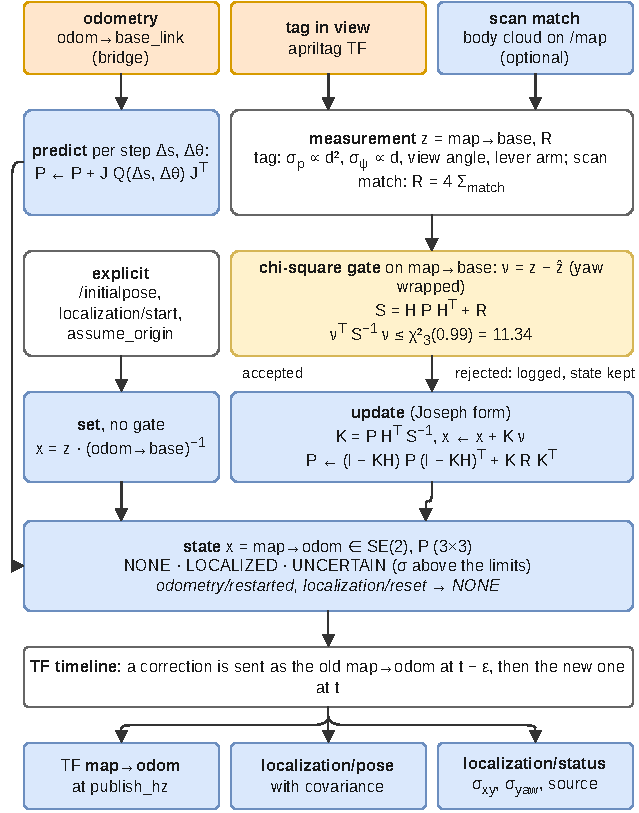
\includegraphics[width=0.62\textwidth]{localization_ekf}
  \caption{EKF over \frm{map}$\to$\frm{odom}: prediction from odometry motion, gated automatic
    corrections, explicit operator input and the TF timeline.}
  \label{fig:m-ekf}
\end{figure}

\subsection{Why}

In 0.1 one tag detection replaced \frm{map}$\to$\frm{odom} directly (finding L1). There was no
covariance, no fusion of detections and no correction between tags; detections were rejected
when the correction itself exceeded 0.5~m or 15° (review \#1), which rejected good fixes far
from the odometry origin and accepted small rotations that moved the robot metres. The errors
of a single detection propagate as
\begin{center}
\begin{tabular}{@{}llr@{}}
  \toprule
  Case & Parameters & Error \\
  \midrule
  PnP of a 16~cm tag, position $\approx d\,\delta$ & $d = 3$~m, $\delta = 3^\circ$ & 15.7~cm \\
  same & $d = 5$~m, $\delta = 2^\circ$ & 17.5~cm \\
  heading of \frm{map}$\to$\frm{odom}, $e_\perp \approx L\,\delta\psi$ & $L = 10$~m,
    $\delta\psi = 1^\circ$ & 17.5~cm \\
  same & $L = 30$~m, $\delta\psi = 1^\circ$ & 52.4~cm \\
  \bottomrule
\end{tabular}
\end{center}

\subsection{State and prediction}

The state is $\vect{x} = (x, y, \psi)$ of $\T{map}{odom}$ with a $3\times3$ covariance
$\mathbf{P}$. Given the odometry pose $\vect{o} = \T{odom}{base}$, the robot pose is
$h(\vect{x}) = \vect{x} \oplus \vect{o} = (x_b, y_b, \psi_b)$ and
\begin{equation}
  \mathbf{H} = \frac{\partial h}{\partial \vect{x}} =
  \begin{bmatrix} 1 & 0 & -(y_b - y) \\ 0 & 1 & x_b - x \\ 0 & 0 & 1 \end{bmatrix}.
\end{equation}
The third column is the lever arm: a rotation of \frm{map}$\to$\frm{odom} moves a robot far from
the \frm{odom} origin by a lot. Odometry motion is counted in steps (a robot standing still
never grows uncertain); for a step of distance $\Delta s$ and rotation $\Delta\theta$ the drift
of the robot pose
\begin{equation}
  \mathbf{Q} = \mathrm{diag}\big(\sigma_s^2\Delta s,\ \sigma_s^2\Delta s,\ \sigma_{\psi s}^2
  \Delta s + \sigma_{\psi\theta}^2 \Delta\theta\big)
\end{equation}
is mapped onto the state, $\mathbf{P} \leftarrow \mathbf{P} + \mathbf{H}^{-1}\mathbf{Q}
\mathbf{H}^{-\top}$. With $\sigma_s = 0.03$~m$/\sqrt{\mathrm{m}}$ the position uncertainty
grows to about 10~cm after 10~m.

\subsection{Update and gate}

A measurement $\vect{z}$ of \frm{map}$\to$\frm{base_link} with covariance $\mathbf{R}$, taken
while the odometry read $\vect{o}$, gives
\begin{equation}
  \vect{\nu} = \vect{z} - h(\vect{x})\ (\text{yaw wrapped}), \qquad
  \mathbf{S} = \mathbf{H}\mathbf{P}\mathbf{H}^\top + \mathbf{R}, \qquad
  d^2 = \vect{\nu}^\top\mathbf{S}^{-1}\vect{\nu}.
\end{equation}
Automatic sources pass only if $d^2 \le \chi^2_3(p)$ ($p$ = \param{estimator.gate_confidence},
0.99: 11.34)~\cite{barshalom2001estimation}. The gate opens as the uncertainty grows after a
long drive and is tight after a correction. An accepted measurement updates
\begin{equation}
  \mathbf{K} = \mathbf{P}\mathbf{H}^\top\mathbf{S}^{-1}, \quad
  \vect{x} \leftarrow \vect{x} + \mathbf{K}\vect{\nu}, \quad
  \mathbf{P} \leftarrow (\mathbf{I} - \mathbf{K}\mathbf{H})\mathbf{P}(\mathbf{I} -
  \mathbf{K}\mathbf{H})^\top + \mathbf{K}\mathbf{R}\mathbf{K}^\top
\end{equation}
(Joseph form, symmetric by construction), followed by a floor on the robot pose covariance
(\param{estimator.min_sigma_xy}, \param{estimator.min_sigma_yaw_deg}) against overconfidence. The reported sigmas are
those of the robot pose, $\mathbf{H}\mathbf{P}\mathbf{H}^\top$: $\sigma_{xy}$ is the square
root of the largest eigenvalue of its position block.

\textbf{States.} \code{NONE} before the first fix (sigmas infinite), \code{LOCALIZED},
\code{UNCERTAIN} when $\sigma_{xy}$ exceeds \param{estimator.max_sigma_xy} or $\sigma_\psi$
exceeds \param{estimator.max_sigma_yaw_deg}.

\subsection{Sources}

\begin{description}
  \item[Tag.] A detection $\T{cam}{tag}$ of a tag with known $\T{map}{tag}$ gives
    \begin{equation}
      \T{map}{base} = \T{map}{tag}\,\big(\T{base}{cam}\,\T{cam}{tag}\big)^{-1},
    \end{equation}
    computed in SE(3) because the optical frame (z forward, x right, y down) is never planar,
    then flattened to $(x, y, \psi)$. Detections farther than \param{tag.max_distance_m} or
    seen more obliquely than \param{tag.max_view_angle_deg} are ignored. The noise grows with
    distance $d$ (at least 0.3~m) and view angle $\alpha$:
    $\sigma_p = \sigma_{p,1}\,d^2/\cos\alpha$, $\sigma_\psi = \sigma_{\psi,1}\,d/\cos\alpha$.
    A heading error rotates the robot about the tag: with $\vect{v}$ the vector from the robot
    to the tag and $\vect{l} = (v_y, -v_x)$,
    \begin{equation}
      \mathbf{R} = \begin{bmatrix} \sigma_p^2\mathbf{I} + \sigma_\psi^2\vect{l}\vect{l}^\top &
      \sigma_\psi^2\vect{l} \\ \sigma_\psi^2\vect{l}^\top & \sigma_\psi^2 \end{bmatrix}.
    \end{equation}
    Far tags therefore count little, and a test with the real optical rotation
    $(-\pi/2, 0, -\pi/2)$ and non-zero yaws checks the geometry (review \#15).
  \item[Pose estimate.] \topic{/initialpose} (RViz 2D Pose Estimate). RViz sends a fixed UI
    covariance whatever the operator meant, so the operator is trusted (5~cm, 2°); a tighter
    covariance from another client (a simulator) is used as given. Applied without gate.
  \item[Scan match] (optional, \param{scan_match.enabled}). The registered body cloud is put
    into the level \frm{odom} with its full 3D pose, a height band above the floor is kept, the
    points are expressed in the planar base frame and matched against \topic{/map} with the
    correlative matcher of \pkg{dharma_utils}~\cite{olson2009csm} (coarse to fine on a
    likelihood field); the covariance of the score surface, scaled by 4, is $\mathbf{R}$.
  \item[Explicit.] \topic{localization/start} (localize from a tag in view),
    \topic{localization/assume_origin} (\frm{map}$\to$\frm{odom} = identity, for a new map) and
    a pose estimate set the state without gate, so a far but consistent tag that the gate
    rejects (after a kidnapping or a wrong pose estimate) still relocalizes on request.
\end{description}

\subsection{Publication without interpolation ramps}

tf2 interpolates between the two samples around a lookup time. If \frm{map}$\to$\frm{odom}
changed between two periodic samples, lookups in that interval would see a blend of the old and
the new value, mapping scans to poses that never existed (findings T1/T3, review \#14). A
correction is therefore published as the previous value at $t - \epsilon$ followed by the new
value at $t$ ($\epsilon = 1$~ms), and periodic samples are strictly increasing in time.

\section{Fiducial tags}

\code{record_tags} averages the map pose of the visible \param{tag.frames} over
\param{tag.record_duration_sec} and merges them into the tags file. It writes the anchors of a
site, so it refuses unless the state is \code{LOCALIZED} and never records the tag the current
\frm{map}$\to$\frm{odom} was derived from (circular, review \#2). Recordings with fewer than
\param{tag.record_min_samples} samples or a larger spread than the limits are refused. It runs
as a session over the node's timers in its own callback group (no sleep in a callback, finding
L2), so \frm{map}$\to$\frm{odom} keeps flowing at \param{publish_hz} while it records. Reads are
tolerant: a corrupt tags file is reported (\texttt{success: false}) and left untouched (review
\#3); every write keeps a \code{.bak}. \code{load_tags} accepts only paths that resolve inside
\param{sites_dir} (review \#12); \code{~} is expanded (review \#11).

\section{Interfaces}

\begin{center}
\begin{tabularx}{\textwidth}{@{}p{0.31\textwidth}p{0.27\textwidth}X@{}}
  \toprule
  Interface & Type & \\
  \midrule
  \topic{localization/start} & Trigger & localize from a tag in view, explicitly \\
  \topic{localization/reset} & Trigger & forget \frm{map}$\to$\frm{odom} \\
  \topic{localization/assume_origin} & Trigger & \frm{map}$\to$\frm{odom} = identity \\
  \topic{localization/record_tags} & Trigger & record the visible tags \\
  \topic{localization/load_tags} & LoadFile & switch the tags file (inside \param{sites_dir}) \\
  \topic{localization/status} & LocalizationStatus & latched: state, source, sigmas, time
    since the last correction \\
  \topic{localization/pose} & PoseWithCovariance\-Stamped & robot pose with covariance \\
  \topic{localization/tag_markers} & MarkerArray & known tags \\
  in: \topic{odometry/restarted}, \topic{/initialpose}, IMU, \topic{/map},
    \topic{/cloud_registered_body} & & \\
  \bottomrule
\end{tabularx}
\end{center}

\section{Parameters}

\readonlynote

% Generated by docs/manual/tools/reference.py; do not edit.
\begin{small}
\begin{longtable}{@{}p{0.28\textwidth}p{0.12\textwidth}p{0.08\textwidth}p{0.11\textwidth}p{0.29\textwidth}@{}}
\toprule
Parameter & Default & Unit & Range & Description \\
\midrule
\endhead
\bottomrule
\endfoot
\multicolumn{5}{@{}l}{\textbf{localization\_node}} \\
\code{sites_dir}$^\dagger$ & \code{~/dharma/map} &  &  & load\_tags paths must be inside \\
\code{tags_file}$^\dagger$ & \code{""} &  &  & tags file at start (empty: none until load\_tags) \\
\code{lio_odom_frame}$^\dagger$ & \code{camera_init} &  &  & LIO world frame \\
\code{lio_body_frame}$^\dagger$ & \code{body} &  &  & LIO body frame (the IMU) \\
\code{imu_frame}$^\dagger$ & \code{livox_imu_frame} &  &  & URDF frame of the LIO body \\
\code{publish_hz}$^\dagger$ & 20 & Hz & 1\,..\,200 & map->odom on /tf \\
\code{pose_hz}$^\dagger$ & 10 & Hz & 0\,..\,100 & localization/pose; 0: off \\
\code{assume_start_origin}$^\dagger$ & false &  &  & the odom origin is the map origin at start (no tag needed) \\
\code{estimator.sigma_xy_per_sqrt_m} & 0.03 & m/sqrt(m) & 0\,..\,1 & position drift: 1-sigma after 1 m of travel \\
\code{estimator.sigma_yaw_deg_per_sqrt_m} & 0.1 & deg/sqrt(m) & 0\,..\,10 & heading drift per metre of travel \\
\code{estimator.sigma_yaw_deg_per_sqrt_rad} & 0.5 & deg/sqrt(rad) & 0\,..\,10 & heading drift per radian turned \\
\code{estimator.gate_confidence} & 0.99 &  & 0.95, 0.99, 0.999 & chi-square gate (3 dof) of automatic corrections \\
\code{estimator.max_sigma_xy} & 0.5 & m & 0.01\,..\,100 & above: state UNCERTAIN (position) \\
\code{estimator.max_sigma_yaw_deg} & 10 & deg & 0.1\,..\,180 & above: state UNCERTAIN (heading) \\
\code{estimator.min_sigma_xy} & 0.01 & m & 0\,..\,1 & floor after a correction (no overconfidence) \\
\code{estimator.min_sigma_yaw_deg} & 0.25 & deg & 0\,..\,10 & heading floor after a correction \\
\code{estimator.motion_step_m} & 0.05 & m & 0.001\,..\,1 & odometry motion counted in steps (jitter-free) \\
\code{estimator.motion_step_deg} & 2 & deg & 0.01\,..\,45 & odometry rotation counted in steps \\
\code{tag.camera_frame}$^\dagger$ & \code{camera_color_optical_frame} &  &  & frame the detector puts the tags under \\
\code{tag.frames} & [\code{base_map}, \code{charging_dock}] &  &  & tag TF frames to record (the detector tag frames) \\
\code{tag.max_age_sec} & 0.5 & s & 0.01\,..\,10 & older detections ignored \\
\code{tag.max_distance_m} & 4 & m & 0.1\,..\,50 & farther tags ignored \\
\code{tag.max_view_angle_deg} & 60 & deg & 1\,..\,89 & tags seen more obliquely are ignored \\
\code{tag.sigma_xy_at_1m} & 0.02 & m & 0.001\,..\,1 & position sigma at 1 m, grows with distance\textasciicircum{}2 \\
\code{tag.sigma_yaw_deg_at_1m} & 1 & deg & 0.01\,..\,30 & heading sigma at 1 m, grows with distance \\
\code{tag.update_hz}$^\dagger$ & 10 & Hz & 0.5\,..\,50 & tag checks \\
\code{tag.min_interval_sec} & 0.5 & s & 0\,..\,60 & per tag, between two fused detections \\
\code{tag.auto_localize} & true &  &  & while not localized: localize from any visible tag \\
\code{tag.auto_correct} & true &  &  & while localized: fuse visible tags through the gate \\
\code{tag.record_duration_sec} & 2 & s & 0.2\,..\,60 & record\_tags \\
\code{tag.record_min_samples} & 5 &  & 1\,..\,1000 & detections needed per tag \\
\code{tag.record_max_std_m} & 0.05 & m & 0.001\,..\,1 & noisier recordings are refused \\
\code{tag.record_max_std_deg} & 3 & deg & 0.01\,..\,45 & noisier recordings are refused (heading) \\
\code{tag.marker_size} & 0.15 & m & 0.01\,..\,2 & tag plate in RViz \\
\code{scan_match.enabled}$^\dagger$ & false &  &  & match the registered cloud against /map \\
\code{scan_match.cloud_topic}$^\dagger$ & \code{/cloud_registered_body} &  &  & deskewed cloud in the LIO body frame \\
\code{scan_match.rate_hz} & 1 & Hz & 0.05\,..\,10 & matches per second, at most \\
\code{scan_match.min_height_m} & 0.1 & m & -1\,..\,5 & band above the floor \\
\code{scan_match.max_height_m} & 1.5 & m & 0\,..\,10 & band above the floor \\
\code{scan_match.max_range_m} & 15 & m & 0.5\,..\,200 & farther points ignored \\
\code{scan_match.xy_window_m} & 0.3 & m & 0.05\,..\,5 & search window \\
\code{scan_match.yaw_window_deg} & 6 & deg & 0.5\,..\,45 & search window \\
\code{scan_match.min_score} & 0.5 &  & 0\,..\,1 & mean likelihood needed \\
\code{scan_match.covariance_scale} & 4 &  & 1\,..\,1000 & inflates the match covariance (correlated points) \\
\code{scan_match.occupied_threshold} & 65 &  & 1\,..\,100 & occupancy value of an obstacle \\
\code{leveling.enabled}$^\dagger$ & true &  &  & level odom with the IMU (off: odom = base) \\
\code{leveling.imu_topic}$^\dagger$ & \code{/livox/imu} &  &  & IMU in the LIO body frame axes \\
\code{leveling.window_sec} & 1 & s & 0.1\,..\,10 & still window \\
\code{leveling.max_rate_deg_s} & 3 & deg/s & 0.1\,..\,90 & still: gyro rate below this \\
\code{leveling.max_accel_spread} & 0.03 &  & 0.001\,..\,0.5 & still: accelerometer std / mean norm below this \\
\code{leveling.max_tilt_deg} & 20 & deg & 1\,..\,60 & larger start tilts are refused (wrong frame?) \\
\code{leveling.timeout_sec} & 15 & s & 0\,..\,600 & then the bridge goes up unleveled; 0: wait \\
\end{longtable}
\end{small}

